\documentclass{article}
\usepackage[utf8]{inputenc}
\usepackage{listings}
\usepackage[margin=1in]{geometry}
\usepackage{parskip}% http://ctan.org/pkg/parskip
\usepackage{hyperref}
\usepackage{float}


\lstset{
language = python,
numbers=left,
frame=single,
breaklines=true
}



\title{A Bayesian Approach to Using Noisy Sensor Data}
\author{Sophia Seitz and Claire Diehl}
\date{October 2014}

\usepackage{natbib}
\usepackage{graphicx}


\begin{document}

\maketitle

\section{The Question}
The output of a sensor, in our case an infrared range finder, is often not as accurate as we would like it to be. In previous classes, we many methods to account for this like averaging many points together. This does not work all that well, and we still wonder whether or not there is a better way, or whether we can do this in a Bayesian way.
\\ \\
We take inspiration from another Bayesian problem, one that uses altered GPS data to better characterize the actual position of a person. After solving this problem, we wanted to see whether this solution would also work to characterize the actual location of a perceived object.

\section{Our Solution}
Before we talk about out Bayesain implementation, we are going to introduce out system. For this case study, we use a range finder mounted to a servo that sends range readings to an arduino. The arduino then communicates the data to python via the serial port. From there, we take the data and update our hypothesis about where there might be something and then finally, we plot a representation of where there are probably objects. 

\begin{figure}[h!]
\centering
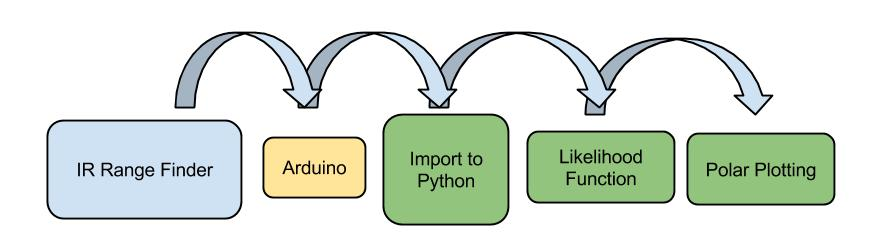
\includegraphics[width=0.6\columnwidth]{BayesSystem.jpg}
\caption{System Diagram}
\label{fig:univerise}
\end{figure}

\subsection{Sensor Setup}
To get the actual sensor data, we mount an infrared range finder to a servo. We then rotate the servo through a range of angles, collect the output of the range finder and the angle, and pass it to our python code running the Bayesian update. Our servo supposedly has a range of 90 degrees, but in the interest of not pushing the servo right to its limit, we sweep through a range of 0 to 85 degrees.

\begin{figure}[h!]
\centering
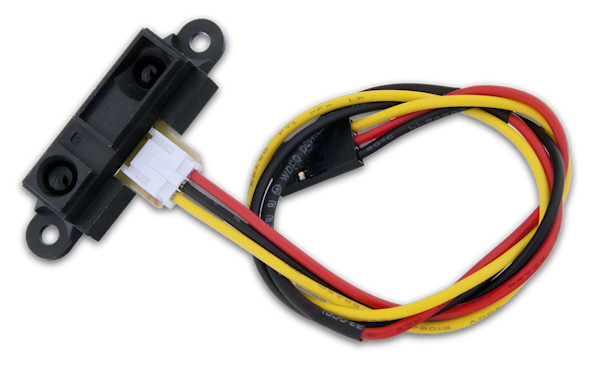
\includegraphics[width=0.3\columnwidth]{IRRANGEFINDER.jpg}
\caption{IR Range Finder similar to the one we used}
\label{fig:rangefinder}
\end{figure}

\begin{figure}[h!]
\centering
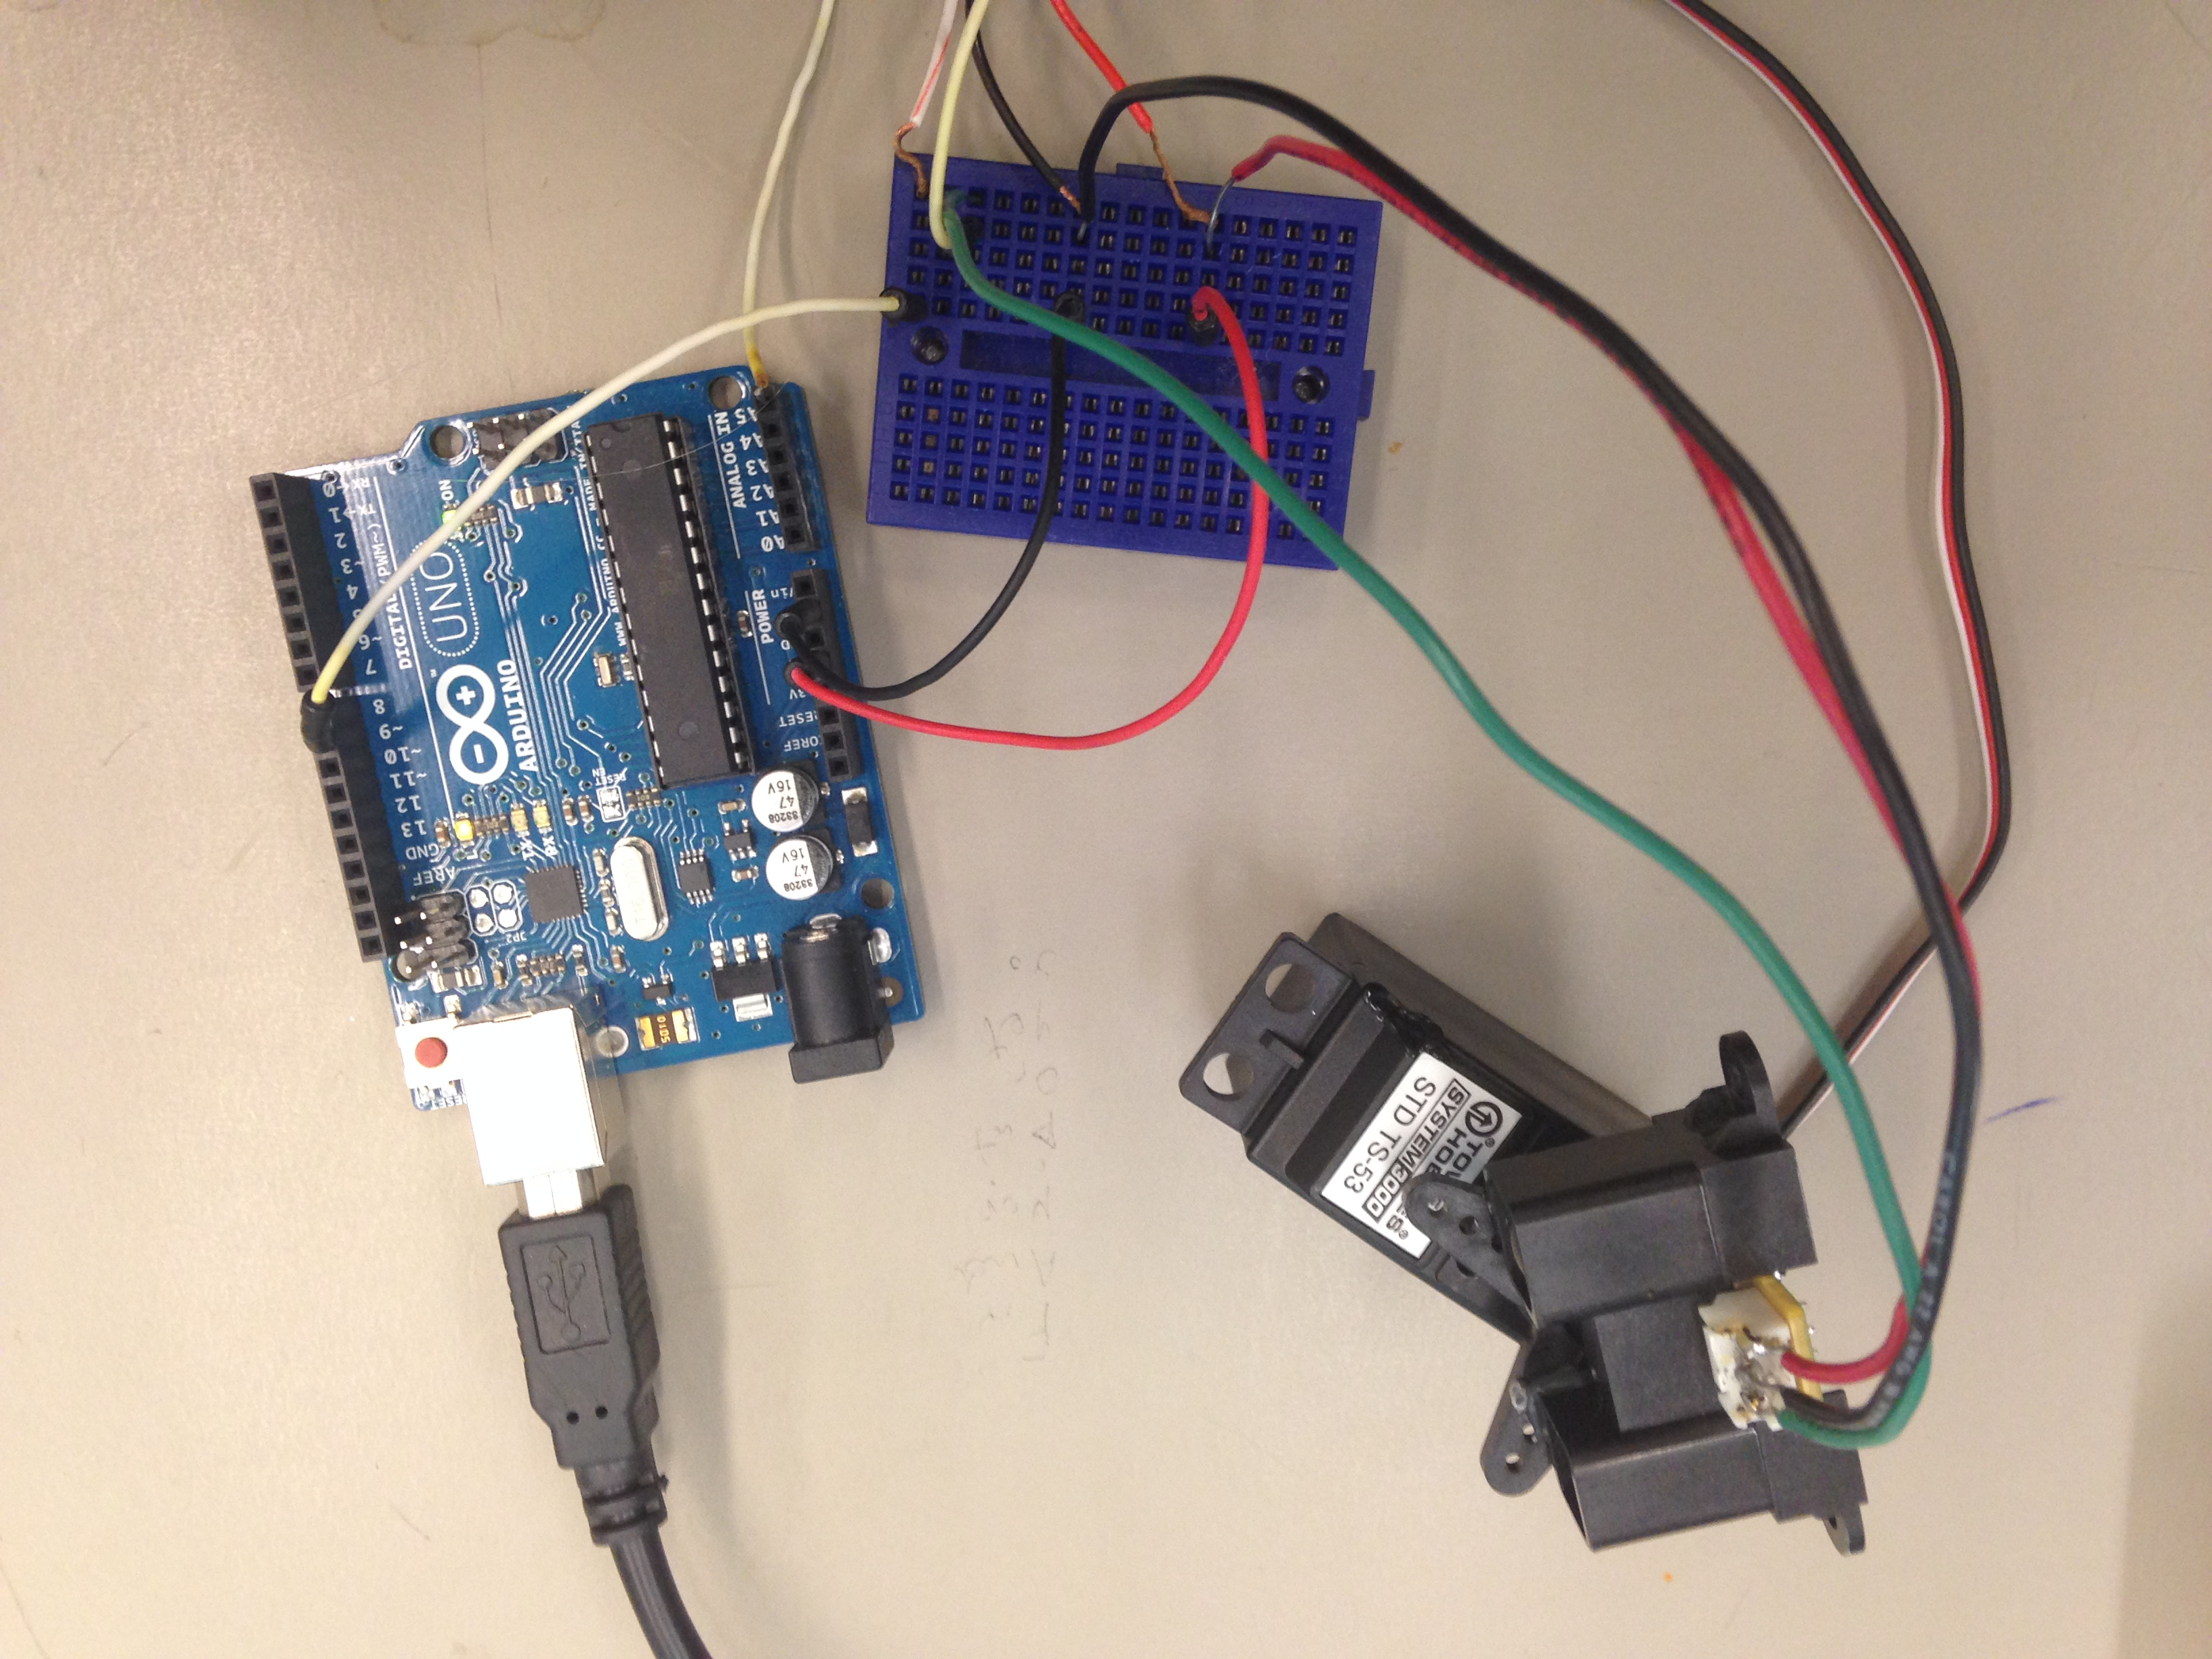
\includegraphics[width=0.3\columnwidth]{IMG_0710.JPG}
\caption{The testing system we used to collect data}
\label{fig:rangefinder}
\end{figure}

\subsection{From Sensor Data to Code}
Before we can implement the Bayesian part of this case study, we have to learn a little about the error of our sensor. We characterize the error for the data by calculating the standard deviation and mean of the error at a series of distance points. Below is a plot of the mean and standard deviation of the error as a function of distance.

\begin{figure}[h!]
\centering
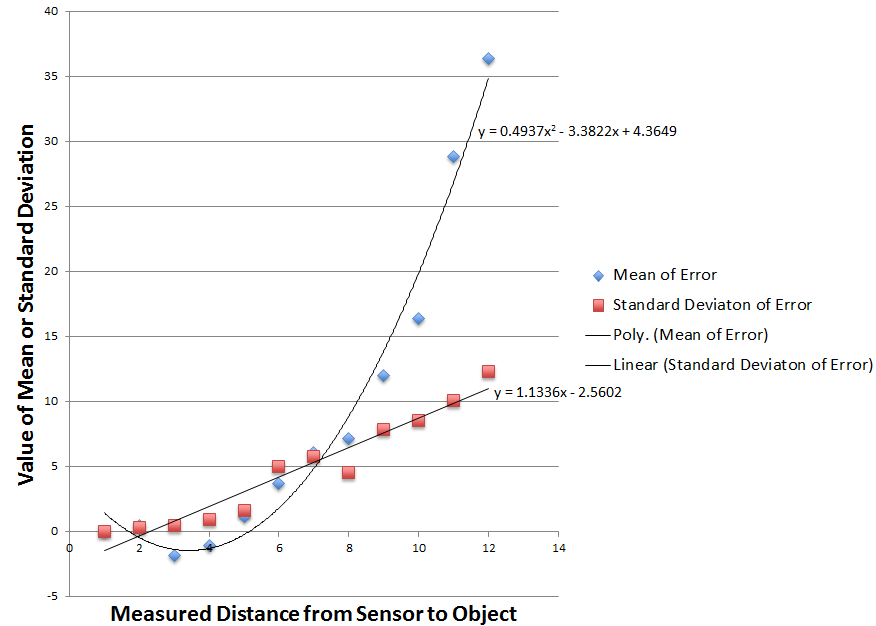
\includegraphics[width=0.7\columnwidth]{calibgraph.PNG}
\caption{A graph of our calibration results}
\label{fig:calibgraph}
\end{figure}

The mean of the error as a function of distance is 

\begin{equation}
mean = 0.0054x^2 - 0.4089x + 6.8076
\end{equation}

and the standard deviation of the error based on the distance from the sensor to an object is 

\begin{equation}
standard deviation  = 0.1211x - 3.2346
\end{equation}

Here, we also assume that the error is normally distributed. This allows us to create a error function based on distance. We use this to calculate potential errors and likelihood of the data.\\
For this case study, we are representing all of our data and hypothesis as radius, angle pairs. It is also worth noting that we assume that there is no error in the angle of the sensor.\\

\subsubsection{Hypotheses}
Okay, enough about all the non-Bayesian parts of this project. In this case study, we have a separate suite of hypotheses for each angle. Within each suite our hypotheses correspond to the distance at which there might be an object. These hypotheses are defined in our code as  
\begin{lstlisting}
rs = np.linspace(minRange,maxRange,numPoints)
thetas = np.arange(0,maxAngle)
suites = []
for theta in thetas:
    suites.append(Lidar(rs))
\end{lstlisting}

Here Lidar is the class that represents our suite of hypotheses.

\subsection{Updating our Hypotheses}
\subsubsection{Data for the Update}
Quick segue back to non-Bayesian things. The data we pass into our likelihood function is all the distances for one sweep of the sensor. This data is of the form of a large tuple containing (85) smaller tuples, where each of those consists of a measured distance and angle. As a note, the sensor does not respond well to distances that are outside its maximum range and often returns "Not a Number", or "NaN". When this happens, we simply set the measured distance to the maximum distance.

\subsubsection{Updating Multiple Suites}
Because we have a suite of hypotheses for each angle, we have to iterate through our data, and choose the appropriate angle suite to update for each piece of data. The code for doing this is

\begin{lstlisting}
def UpdateSuites(suites, data):
    for measurement in data:
        r = measurement[0]
        theta = measurement[1]
        suite = suites[theta]
        suite.Update(r)
\end{lstlisting}

\subsubsection{Likelihood Function}
Our likelihood function is as follows. We use the error that we characterized above to compute the likelihood that we get a given measurement if we have an object at our hypothesis. 

\begin{lstlisting}
def Likelihood(self, data, hypo):
    #Computes the likelihood of the data under the hypothesis.
    #hypo: hypothetical distance
    #data: measured distance.
    
    error = data - hypo
    #Mean and STD calculated based on distance 
    mean = 0.0054*hypo**2 - 0.4089*hypo + 6.8076
    std = 0.1211*hypo - 3.2346

    like = thinkbayes2.EvalNormalPdf(error, mean, std)
    if math.isnan(like):
        like = 5e-50

    return like
\end{lstlisting}

\subsection{Polar Plotting}
After calculating likelihoods and updating our hypotheses, we would like to present our data in an understandable way. Funnily enough, we don't think thinkplot includes anything about plotting in polar coordinates so we made our own because polar plotting is the easiest method for us to communicate our data.
\begin{lstlisting}
def plotPolar(suites):
    rsarray = np.linspace(minRange,maxRange,numPoints)
    thetasarray = np.arange(0,maxAngle)
    thetasradarray = np.radians(thetasarray)

    rs,thetasrads = np.meshgrid(thetasradarray, rsarray)
    likes = np.zeros((rsarray.size,thetasarray.size))

    for theta in thetasarray:
        currentSuite = suites[theta]
        for indexr,r in enumerate(rsarray):
            likes[indexr][theta] = currentSuite.Prob(r)

    fig, ax = plt.subplots(subplot_kw=dict(projection='polar'))
    ax.contourf(rs,thetasrads, likes)

    plt.show()

\end{lstlisting}

\section{Our Results}
To test how well our Bayesian system works, we scan a corner of the walls in an East Hall team room. Here is our testing setup. \\

\begin{figure}[H]
\centering
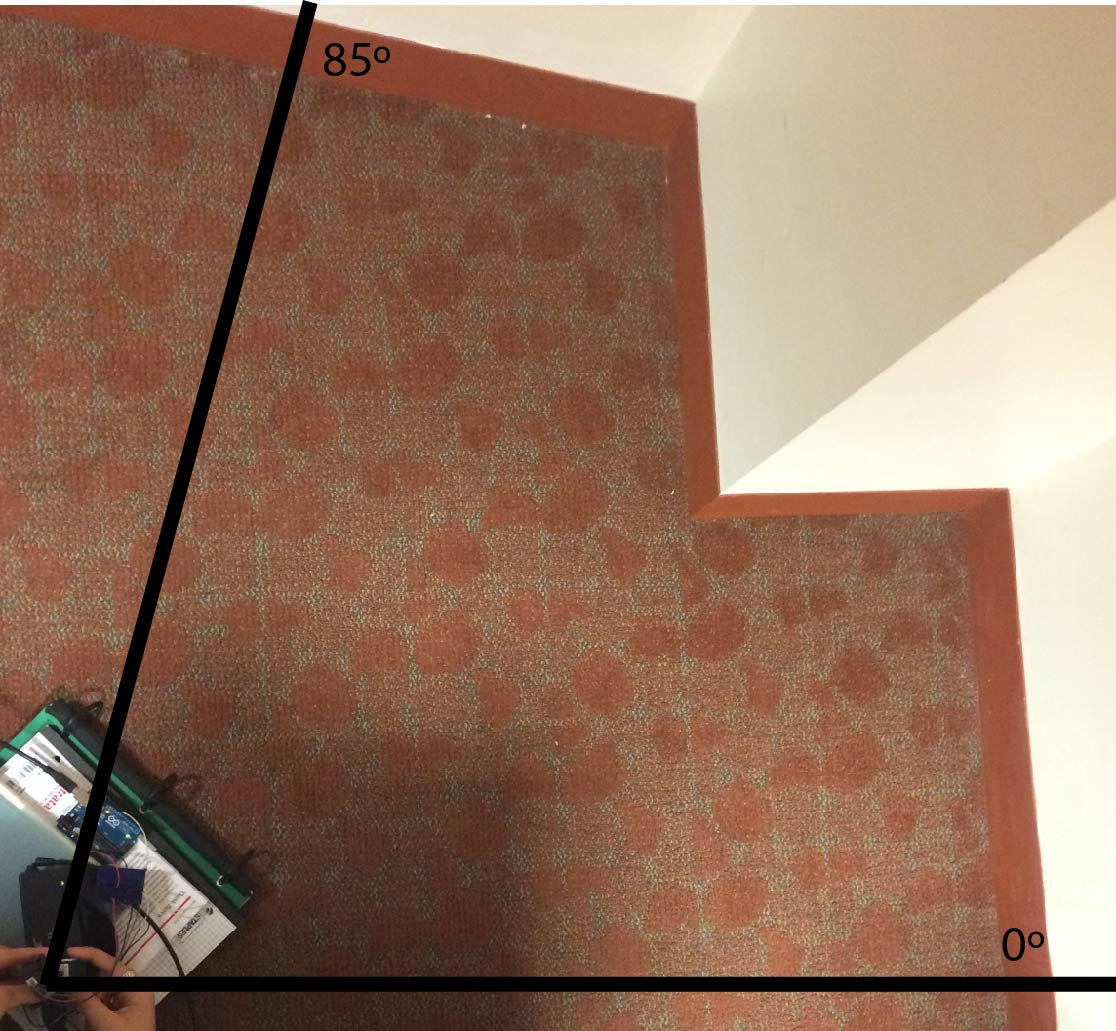
\includegraphics[width=0.6\columnwidth]{corners.jpg}
\caption{The testing setup}
\label{fig:testing}
\end{figure}

We scanned this area 5 times, and below are each of the outputs of our likelihood function.\\

\begin{figure}[H]
\centering
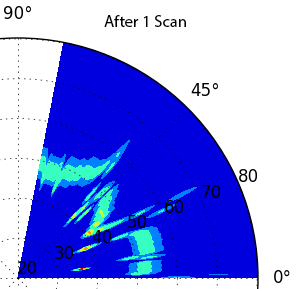
\includegraphics[width=0.4\columnwidth]{teamroomcorner1.png}
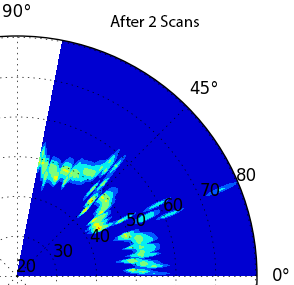
\includegraphics[width=0.4\columnwidth]{teamroomcorner2.png}
\end{figure}
\begin{figure}[H]
\centering
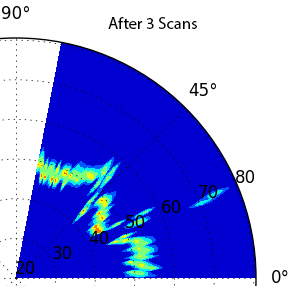
\includegraphics[width=0.4\columnwidth]{teamroomcorner3.png}
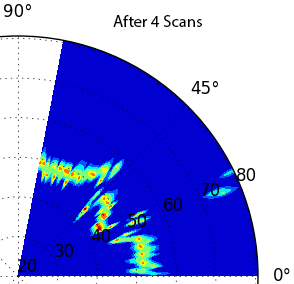
\includegraphics[width=0.4\columnwidth]{teamroomcorner4.png}
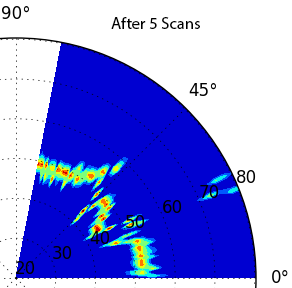
\includegraphics[width=0.4\columnwidth]{teamroomcorner5.png}
\caption{Our scans of set of corners in an East Hall team room}
\label{fig:Corner}
\end{figure}

Each time the general shape of the graph looks the same. Every time that we scan, we are more and more sure that there is a set of three corners as well as the precise location of these obstacles. There is still a little noise right around the sharp corners, but that's reasonable. Corners are hard.  \\

\section{Our Interpretation}
Bayesian is the best!\\
Maybe. We do not compare this data to another method of calculating the probable location of the wall and are not completely convinced that this solution is better than an average of multiple scans or even just the raw data. However, in a short number of scans we can relatively accurately map a difficult set of corners with decent probability. This proves that Bayesian is, at very least, a usable solution to this question.

\section{References}
Our repo: \href{https://github.com/phiaseitz/CompBayesCaseStudy}{CompBayesCaseStudy}\\
\url{https://github.com/phiaseitz/CompBayesCaseStudy}\\ \\
Reference for arduino control of IR sensor and motor, as well as communication with python: \href{https://github.com/JPWS2013/PoE_F2013/tree/master/Lab_1}{PoE Lab}\\
\url{https://github.com/JPWS2013/PoE_F2013/tree/master/Lab_1}\\


\end{document}
